\documentclass[12pt]{article}
\usepackage[utf8]{inputenc}
\usepackage{enumerate}
\usepackage{float}
\usepackage{graphicx}
\usepackage{listings}
\usepackage{multicol}
\usepackage{multirow}
\usepackage[table]{xcolor}

\title{[CO-460] Computer Architecture Assignment}
\author{Rahul Jha \thanks{S.No = 19 Faculty Number = 16LEB167}}
\date{\today}

\begin{document}

\maketitle

\section{5-bit ALU}

\subsection{Question}
Design a 5 bit ALU, which can perform following operations (use carry select
adder).

\begin{multicols}{2}
  \begin{enumerate}[i]
      \item Arithmetic Addition
      \item Arithmetic Subtraction
      \item Logical Shift Left
      \item Logical Shift Right
      \item Rotate left by 1
      \item Rotate Right by 1
      \item AND
      \item OR
      \item XOR
      \item NOR
      \item NAND
      \item XNOR
      \item $ A > B $
      \item $ A < B $
      \item $ A = B $
  \end{enumerate}
\end{multicols}

\newpage

\subsection{Design}

The truth table for the ALU is as follows:

\begin{table}[h]
\centering
\begin{tabular}{c c c c c}
    \textbf{Index} & \textbf{Group} & \textbf{S[3:0]} &
    \textbf{Function} & \textbf{Description} \\
    \hline
    0 & \multirow{2}*{Arithmetic} &
      0000 & $ A + B $ & Arithmetic addition \\
    1 & & 0001 & $ A - B $ & Arithmetic subtraction \\
    \hline
    2 & \multirow{4}*{Shift} &
      0010 & $ A << 1 $ & Logical left shift \\
    3 & & 0011 & $ A >> 1 $ & Logical right shift \\
    4 & & 0100 & $ A <<< 1 $ & Rotate left \\
    5 & & 0101 & $ A >>> 1 $ & Rotate right \\
    \hline
    6 & \multirow{6}*{Logical} &
      0110 & $ A \wedge B $ & AND \\
    7 &  &  0111 & $ A \vee B $ & OR \\
    8 &  &  1000 & $ A \oplus B $ & XOR \\
    9 &  &  1001 & $ A \downarrow B $ & NOR \\
    10 & &  1010 & $ A \uparrow B $ & NAND \\
    11 & &  1011 & $ A == B $ & XNOR \\
    \hline
    13 & \multirow{3}*{Comparison} &
      1100 & $ A > B $ & Greater than \\
    14 & & 1101 & $ A < B $ & Lesser than \\
    15 & & 1110 & $ A = B $ & Equal To \\
    \hline
    16 & Forbidden & 1111 & -- & -- \\
\end{tabular}
\caption{Truth Table}
\end{table}

\newpage

\subsection{Verilog Code}
\lstinputlisting[numbers=left, language=verilog]{alu.v}

\newpage

\subsection{Writing the Test Bench}
\lstinputlisting[numbers=left, language=verilog]{alu_tb.v}

\newpage

\subsection{Results}

Compiling the above test bench with \texttt{iverilog} (\textit{``Icarus Verilog
Compiler"}) using command:

\begin{verbatim}
  $ iverilog -o alu.out alu_tb.v && ./alu.out
\end{verbatim}

gives us the following results:

\begin{verbatim}
A = 26, B = 17, S =  0, Y = 11 (Cout = 1)
A = 26, B = 17, S =  1, Y =  9 (Cout = 0)
A = 26, B = 17, S =  2, Y = 20 (Cout = 1)
A = 26, B = 17, S =  3, Y = 13 (Cout = 0)
A = 26, B = 17, S =  4, Y = 20 (Cout = 0)
A = 26, B = 17, S =  5, Y = 13 (Cout = 0)
A = 26, B = 17, S =  6, Y = 16 (Cout = 0)
A = 26, B = 17, S =  7, Y = 27 (Cout = 0)
A = 10, B =  1, S =  8, Y = 11 (Cout = 0)
A = 11, B =  1, S =  9, Y = 20 (Cout = 0)
A = 11, B =  1, S = 10, Y = 30 (Cout = 0)
A = 11, B =  1, S = 11, Y = 21 (Cout = 0)
A = 11, B =  1, S = 12, Y =  1 (Cout = 0)
A =  3, B = 17, S = 13, Y =  1 (Cout = 0)
A =  2, B = 11, S = 13, Y =  1 (Cout = 0)
A = 11, B = 11, S = 14, Y =  1 (Cout = 0)
A = 31, B = 31, S = 15, Y =  z (Cout = 0)
\end{verbatim}

\subsubsection{Visualizing Output}
The output (dumped in \texttt{alu.vcd}) file can be visualized using
\textit{``gtkwave"}, which produces the following results:

\begin{figure}[H]
  \centering
  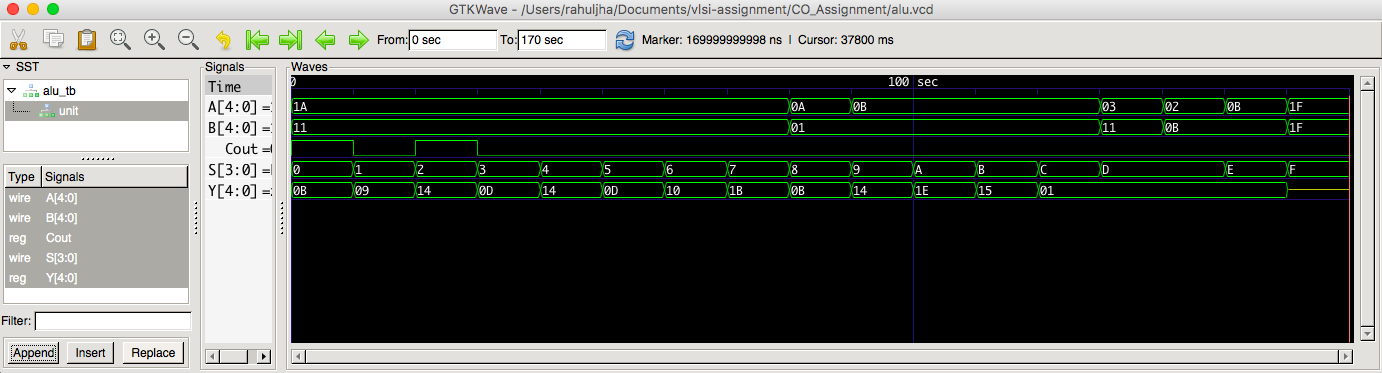
\includegraphics[width=\columnwidth]{img/alu.png}
  \caption{\texttt{alu.vcd} visualized in ``gtkwave".}
  \label{fig:alu}
\end{figure}

\end{document}
